\section{Обзор}
\lstset{basicstyle=\normalsize\ttfamily, columns=fullflexible}
В данном обзоре рассматриваются некоторые подходы к заданию принтеров и форматеров, а также плагин Grammar-Kit для IntelliJ IDEA, позволяющий по БНФ-грамматике задавать синтаксический анализатор целевого языка.
Используемые плагином грамматики рассматриваются на примере грамматики языка While~\cite{paper:nielson}.

\subsection{Подходы к заданию принтеров и форматеров}
Рассмотрим некоторые подходы к заданию принтеров и форматеров.
\subsubsection{Задание форматеров по описанию синтаксиса.}%Язык описания синтаксиса}
Существуют различные подходы к заданию принтеров для целевого языка.
Один из них описан в~\cite{paper:tbe}.
Авторы предлагают язык описания синтаксиса, по которому можно получить и синтаксический анализатор, и принтер для языка.
Описание синтаксиса состоит из правил, которые схожи с правилами формальных грамматик, но которые также задают и стиль форматирования для данной структуры языка.
Приведенное ниже правило вывода описывает основные арифметические выражения:
{
    \lstinputlisting{Ozernykh/codes/tbeif.txt}
    %% =================================================
    %% ПРИМЕР ПОИНТЕРЕСНЕЕ
    %% непонятно, как задаются условия форматирования
    %% =================================================
}
\noindent
Первое преобразование определяет шаблон для выражений, состоящих из чисел.
Остальные преобразования задают шаблоны для операций сложения и вычитания.
Каждое из них состоит из двух меток \lstinline{<Exp>} для подстановки выражений, арифметического знака, а также двух пробелов вокруг этого знака.
Само правило явно задает способ, которым будут отформатированы арифметические выражения полученного языка.
%При дальнейшем форматировании программ на данном языке, арифметические выражения будут иметь вид, задаваемый правилом.
Вместо пробелов можно также указать табуляции и/или переносы строк.
Недостатком данного подхода является то, что правила форматирования задаются заранее, и, чтобы их изменить, необходимо менять описание синтаксиса языка.
Кроме того, каждое такое правило задает единственный вариант форматирования данной структуры.

%\subsubsection{}
Наиболее близкий к нашей работе метод описан в~\cite{paper:asf-sdf}.
Принтер языка может быть получен по ASF+SDF--описанию языка~\cite{paper:klint}, что представляет собой контекстно-свободную грамматику.
При этом правила форматирования не указываются.
Недостатком данного подхода является то, что при генерации принтера задается базовый стиль форматирования, и, чтобы его изменить, необходимо редактировать сгенерированный код, тогда как подход с использованием синтаксических шаблонов позволяет пользователю декларативным образом настраивать принтер.

\subsubsection{Форматеры, встроенные в IDE.}
Также широко распространены форматеры, встроенные в IDE.
Они используют множество настроек для задания стиля форматирования (рис.~\ref{ov:settings}).
Среди них: тип и размер отступов, расположение фигурных скобок в C-подобных языках, политика переноса списочных выражений на новую строку и десятки других.
Набор этих настроек выбирается разработчиком форматера на основе его представлений о возможных стилях кодирования для целевого языка.
Такие форматеры обычно тесно интегрированы с IDE, имеют высокую скорость работы, и их выразительности, как правило, достаточно для задания необходимого стиля форматирования.
Однако для поддержки нового языка необходимо определить нужный набор настроек и вручную реализовать форматер.
В случае, если пользователю необходимо придерживаться стиля кодирования некоторой существующей кодовой базы, то ему нужно самостоятельно определить значения этих настроек.
Данный недостаток отсутствует в работе~\cite{paper:sformatters}, где авторы предлагают инструмент, позволяющий получить некоторые настройки форматера из существующего программного кода.
Недостатком подхода является то, что число этих настроек невелико: система позволяет определять только стиль отступов, стили именования идентификаторов, необходимое количество комментариев.
Другой подход~\cite{blog:genformat} предлагает использование генетического алгоритма 
%\footnote{\texttt{https://en.wikipedia.org/wiki/Genetic\textunderscore algorithm}} 
для поиска настроек форматера в исходном коде программ на языке C.

%и в работе\footnote{\texttt{https://blog.jetbrains.com/clion/2015/11/applying-genetic-algorithms-to-automatic-code-formatting/}}. 
%Они представляют собой способы автоматического вычленения настроек форматирования из программного кода.
\begin{figure}[t]
    \centering
    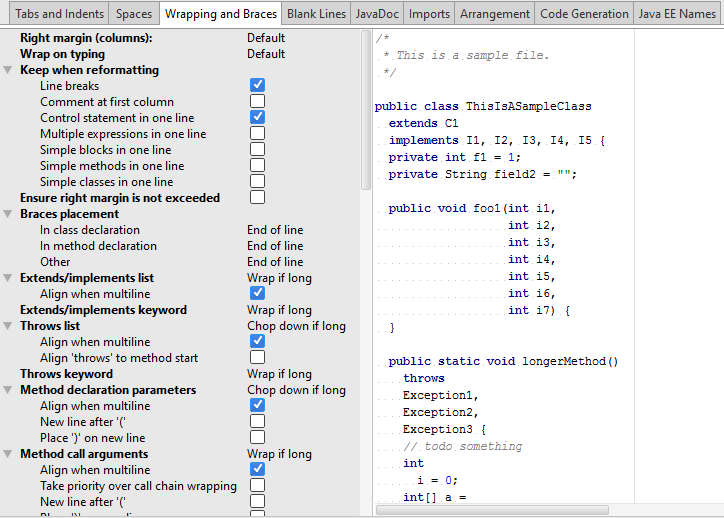
\includegraphics[width=.9\textwidth]{Ozernykh/images/settingsjava.PNG}
    \caption{Настройки форматера языка Java в IntelliJ IDEA}
    \label{ov:settings}
\end{figure}

\subsection{Grammar-Kit}
Как уже было отмечено, для поддержки нового языка в платформе IntelliJ IDEA необходимо разработать синтаксический анализатор.
Для его генерации можно использовать плагин Grammar-Kit.
В качестве системы описания синтаксиса языка используется БНФ-грамматика.
Результатом работы плагина является код синтаксического анализатора и иерархия классов внутреннего представления. %(для IntelliJ IDEA~--- \emph{PSI-классов}).%PSI-классов.
%PSI-классом является каждая структура языка, вместе они образуют иерархию.

%Кроме того, при реализации поддержки нового языка в платформе возникает потребность в форматере.
%Мы хотим задавать принтер для языка, используя его грамматику.
% что тут еще описывать?
%\subsection{Грамматика языка While}
%Для апробации метода, описанного в~\cite{paper:while}, использовался язык While, поэтому будем рассматривать грамматики, с которыми работает Grammar-Kit, на примере грамматики языка While.
Рассмотрим грамматику языка While, для которого производилась апробация метода, описанного в~\cite{paper:while}.
%Рассмотрим БНФ-грамматику, использующуюся в плагине Grammar-Kit на примере грамматики языка While (рис.~\ref{ov:whileBnfFull}).
%\begin{figure}[p]
%\fvset{frame=lines,framesep=5pt}
While~--- язык программирования, содержащий следующие конструкции: чтение из стандартного потока (\lstinline{read}) и запись в стандартный поток (\lstinline{write}), оператор ветвления (\lstinline{if}), цикл с предусловием (\lstinline{while}); процедуры (\lstinline{proc}), бинарные выражения (\lstinline{binary_expr}), в том числе булевы (\lstinline{binary_bexpr}) и т. д.
% (рис.~\ref{ov:whileI},~\ref{ov:whileII},~\ref{ov:whileIII}).
\begin{figure}[h]
 %   \begin{pyglist}[numbers=left,numbersep=5pt]%, basicstyle=\ttfamily]
    \begin{lstlisting}[numbers=left, numbersep=3pt, basicstyle=\ttfamily\small, numberstyle=\tiny, frame=bottom, language={}]
whileFile  ::= proc_list stmt_list
stmt_list  ::= stmt*
proc_list  ::= procedure*
stmt       ::= skip|assign|if|while|write|read
skip       ::= 'skip' ';'
write      ::= 'write' '(' expr ')' ';'
read       ::= 'read' '(' id ')' ';'
assign     ::= id ':=' expr ';'
if         ::= 'if' '(' bexpr ')' 'then' stmt_list ('else' stmt_list)? 'fi'
while      ::= 'while' '(' bexpr ')' 'do' stmt_list 'od'
procedure  ::= 'proc' id '(' param_list ')' stmt_list 'endp'
param_list ::= ref_expr? (',' ref_expr)*
...
 \end{lstlisting}
    \caption{Грамматики языка While. Операторы языка}
    \label{ov:whileI}
\end{figure}
\noindent
На рис.~\ref{ov:whileI} представлена часть грамматики языка While, задающая множество операторов.
Рассмотрим правило грамматики, задающее оператор ветвления.
Правая часть правила состоит из терминалов \lstinline{'if'}, \lstinline{'then'} \lstinline{'('} и др.; нетерминалов: \lstinline{bexpr}, \lstinline{stmt_list}, а также условного вхождения \lstinline{('else' stmt_list)?} (то есть конструкция может отсутствовать в программах на данном языке).
Некоторые правила грамматики имеют модификаторы, которые используются для дополнительных указаний генератору синтаксического анализатора (рис.~\ref{ov:whileII}).
\begin{figure}[h]
    %\begin{pyglist}[numbers=left,numbersep=5pt]
    \begin{lstlisting}[numbers=left, numbersep=3pt, basicstyle=\ttfamily\small, numberstyle=\tiny, frame=bottom, language={}]
...
fake ar_op        ::= plus_op|mul_op
fake binary_expr  ::= expr ar_op expr 

expr              ::= factor plus_expr *
left plus_expr    ::= plus_op factor
plus_op           ::= '+'|'-'
private factor    ::= primary mul_expr *
left mul_expr     ::= mul_op primary
mul_op            ::= '*'|'/'|'%'
private primary   ::= literal_expr | ref_expr | paren_expr
paren_expr        ::= '(' expr ')'
ref_expr          ::= id
literal_expr      ::= number

fake bl_op        ::= or|and
fake binary_bexpr ::= bexpr bl_op bexpr
...
    \end{lstlisting}
    %\end{pyglist}
    \caption{Грамматика языка While. Выражения с модификаторами}%?
    \label{ov:whileII}
\end{figure}
\noindent
Модификатор \lstinline{fake} указывает системе, что не нужно генерировать код синтаксического анализатора для обработки данной структуры, однако генерируется иерархия классов внутреннего представления, \lstinline{private} указывает, что не будет сгенерирована иерархия классов, \lstinline{left} используется для поддержки левоассоциативности, а также некоторые другие\footnote{Посмотреть полный список можно по адресу \texttt{https://github.com/JetBrains/Grammar-Kit}}.
Модификатор \lstinline{private} используется для правил грамматики, которые не имеют представления в синтаксическом дереве.
Среди них те, которые используются для устранения левой рекурсии.
%которые не влияют на синтаксис языка, например, такие, которые используются для устранения левой рекурсии.
Например, на рис.~\ref{ov:whileExpr} представлено описание правил с рис.~\ref{ov:whileII} (строки 5--14), но в более естественной для человеческого восприятия леворекурсивной форме.
\begin{figure}[h]
    %\lstinputlisting{codes/whileExpr.txt}
    %\begin{pyglist}[numbers=left,numbersep=5pt]
    \begin{lstlisting}[numbers=left, numbersep=3pt, basicstyle=\ttfamily\small, numberstyle=\tiny, frame=bottom, language={}]
expr         ::= plus_expr | mul_expr | paren_expr | ref_expr | literal_expr
plus_expr    ::= expr plus_op expr
plus_op      ::= '+'|'-'
mul_expr     ::= expr mul_op expr
mul_op       ::= '*'|'/'|'%'
paren_expr   ::= '(' expr ')'
ref_expr     ::= id
literal_expr ::= number
    \end{lstlisting}
    %\end{pyglist}
    \caption{Грамматики языка While. Выражения в естественной леворекурсивной форме}
    \label{ov:whileExpr}
\end{figure}
\noindent
Однако грамматика, с которой работает Grammar-Kit, не должна содержать леворекурсивных правил.
Устраняя левую рекурсию, мы получим описание выражений на рис.~\ref{ov:whileII} (строки 5--14).
Кроме того, появляются новые правила, которые с точки зрения синтаксического анализа (а следовательно, и форматирования) являются избыточными.
В данном случае такими являются \lstinline{factor} и \lstinline{primary} на рис.~\ref{ov:whileII}.
\begin{figure}[b]
    %\begin{pyglist}
    \begin{lstlisting}[numbers=left, numbersep=3pt, basicstyle=\ttfamily\small, numberstyle=\tiny, frame=bottom, language={}]
{   parserClass="com.intellij.whileLang.parser.WhileParser"
    psiClassPrefix="Psi"
    psiImplClassSuffix="Impl"
    psiPackage="com.intellij.whileLang.psi.impl"
    tokens=[...]
    ...
}
...
    \end{lstlisting}
    %\end{pyglist}
    \caption{Заголовок файла с грамматикой}
    \label{ov:whileIII}
\end{figure}
% про left
Каждый файл с грамматикой языка содержит в себе заголовок, в котором описывается различная дополнительная информация: используемые в сгенерированных файлах классы, префиксы и суффиксы сгенерированных классов внутреннего представления, Java-пакеты, множество терминальных символов грамматики (\emph{tokens}) и др. (см рис.~\ref{ov:whileIII}).




